\chapter{Background Foundations} \label{chap2}
The main aim of this chapter is to provide some background concepts 
in property verification that are necessary for developing the foundations of 
the work. We will begin with a background study of the basic building blocks  
of the validation flow that are at the heart of Figure~\ref{fig1.2}
and proceed to present an extensive survey of 
methodologies and tools that have made property verification a successful 
technology today.

\noindent
Property verification is predominantly used in two forms in pre-silicon
validation, namely (a) static Formal Property Verification (FPV), and 
Dynamic Property Verification (DPV). In the following sections, 
we will highlight the concepts behind each of the above technologies. 

\section{Specification Development} \label{sec2.1}
The first task in all forms of property verification is the development of
the formal specification in a specification language.
This is a non-trivial task and typically done by a few specialized 
verification engineers today. In the following subsections, we first 
present a brief discussion of specification languages, their features and 
enhancements.

\subsection{Temporal Logics} \label{sec2.1.0}
\noindent
Property specification languages derive their formalism from few specific
types of logics called {\em temporal logics}.  The main feature of temporal 
logics, which makes them useful in practice for design verification, is the 
ability to describe sequences of events over time. Temporal logics are 
extensions
of propositional logic, where in addition to the familiar Boolean operators
(AND, OR, and NOT) we have {\em temporal operators} that allow us to specify
constraints on the truth of the propositions over time. In other words,
temporal logics allow us to specify properties that describe the behavior of
a circuit over time, across cycle boundaries. 

\noindent
Temporal logics were originally developed by philosophers for reasoning 
about events across temporal worlds
using natural language. Pnueli was the first to use Linear Temporal Logic
(LTL) to reason about the temporal behavior of concurrent
programs~\cite{pnueli:77}. In~\cite{clarke:86}, Clarke, Emerson and Sistla 
proposed the use of Computation Tree Logic (CTL) for the specification and 
verification of branching time properties. In the following discussion, 
we discuss the syntax and semantics of LTL, since we use it as the primary 
specification language in this work.

\subsection{Linear Temporal Logic} \label{sec2.1.1}
To get a first-cut workable understanding of temporal logics, we 
will consider the basic temporal operators in Linear Temporal Logic (LTL) 
and their meaning. The operators are
interpreted over a state machine -- the purpose of verification is to interpret
the properties over the state machine representation of the design
implementation. The basic set of temporal operators in LTL are:
\begin{description}

\item[$X$: {\em The next-time operator}] The property, $X\varphi$, is true
    at a state of the underlying design-under-test (DUT) if $\varphi$
    is true in the next cycle, where $\varphi$ may be another temporal
    property or a Boolean property over the state bits.

\item[$F$: {\em The future operator}] The property, $F\varphi$, is true at a
    state if $\varphi$ is true {\em sometime} (at some state) in the
    future.

\item[$G$: {\em The global operator}] The property, $G\varphi$, is true at a
    state if $\varphi$ is true {\em always} in the future.

\item[$U$: {\em The until operator}] The property, $\varphi\ U\ \psi$ is
    true at a state if $\psi$ is true at some future state, $t$, and
    $\varphi$ is true at all states leading up to $t$.

\end{description}
\noindent
The operators $X$ and $U$ are the only fundamental temporal operators -- $F$
and $G$ can be derived from combinations of $U$ and Boolean operators. 
The following example illustrates some of the basic operators.

\begin{example} \label{ex2.1}
{\em
Let us consider the specification of a 2-way priority arbiter having the
following interface:
\begin{tabbing}
aa \= aa \= aa \= \kill
\> mem-arbiter( input $r_1$, $r_2$, $clk$, output $g_1$, $g_2$ )
\end{tabbing}
$r_1$ and $r_2$ are the request lines, $g_1$ and $g_2$ are the corresponding
grant lines, and $clk$ is the clock on which the arbiter samples its inputs
and performs the arbitration. We assume that the arbitration decision for the
inputs at one cycle is reflected by the status of the grant lines in the
next cycle. Let us suppose that the specification of the arbiter contains
the following requirements:
\begin{enumerate}
\item Request line $r_1$ has higher priority than request line $r_2$. Whenever
    $r_1$ goes high, the grant line $g_1$ must be asserted for the
    next two cycles.
\item When none of the request lines are high, the arbiter parks the grant
    on $g_2$ in the next cycle.
\item The grant lines, $g_1$ and $g_2$, are mutually exclusive.
\end{enumerate}
\noindent
This constitutes the specification of the arbiter.

\noindent
We now describe how to express the above requirements 
using LTL. The first property may be written as:
{\tt
\begin{tabbing}
a\= aa\= aaa\= aaaa \= aaaaa \= aaaaaa\= aaaaaaa\= \kill
\>\>\>\>\>\> P1: G ($r_1$ $\Rightarrow$  X $g_1$ $\land$  XX $g_1$)
\end{tabbing}
}
\noindent
The subformula $r_1 \Rightarrow\  Xg_1\ \land\  XXg_1$ says: {\em If $r_1$
is high in a cycle, then $g_1$ must be true in the next cycle and $g_1$
must be true in the next next cycle, that is, the second cycle after the
initial cycle}. The $G$ operator says that the
above subformula must hold on all cycles. This does not mean that $r_1$
has to be true in all states -- those states where $r_1$ is low satisfy the
implication {\em vacuously}, since $r_1 \Rightarrow\  Xg_1\ \land\  XXg_1$
evaluates to true regardless of the value of $g_1$ in the next two cycles.

\noindent
The second property can be written as:
{\tt
\begin{tabbing}
a\= aa\= aaa\= aaaa \= aaaaa \= aaaaaa\= aaaaaaa\= \kill
\>\>\>\>\>\> P2: G ($\neg r_1$ $\land$ $\neg r_2$ $\Rightarrow$  X $g_2$)
\end{tabbing}
}
\noindent
The meaning of this property is exactly as before -- {\em in every state,
if both $r_1$ and $r_2$ are low, then $g_2$ must be high in the next cycle}.

\noindent
The third property can be written as: 
{\tt
\begin{tabbing}
a\= aa\= aaa\= aaaa \= aaaaa \= aaaaaa\= aaaaaaa\= \kill
\>\>\>\>\>\> P3: G ($\neg g_1$ $\lor$ $\neg g_2$)
\end{tabbing}
}
\noindent
This property says: {\em always at least one among $g_1$ and $g_2$ must be
low}, which expresses the mutual exclusion requirement.
} $\Box$
\end{example}

\subsubsection{Linear Temporal Logic: Syntax} \label{sec2.1.1.1}
We can define the syntax of LTL recursively as follows:
\begin{itemize}

\item All Boolean formulas over the state variables are LTL properties.

\item If $f$ and $g$ are LTL properties, then so are: $\neg f$, $Xf$, and
	$f\ U\ g$.

\end{itemize}

\subsubsection{Linear Temporal Logic: Semantics} \label{sec2.1.1.2}
To explain the semantics of Linear Temporal Logics formally, we will need a 
model of the underlying state machine of the design-under-test, 
popularly known as the Kripke structure in the verification community.
Formally, we define a Kripke structure as a tuple,
$J = \langle S, {\cal AP}, \tau, s_0, {\cal F} \rangle$, where:
\begin{itemize}
\item $S$ is a finite set of states,
\item ${\cal AP}$ is a set of atomic propositions labeling each state
       $s \ \in \ S$,
\item $\tau\ \subseteq S \times S$ is the transition
      relation, which must be total (for all states $s_i\ \in\ S$,
      there exists a state $s_j\ \in\ S$ such that
      $(s_i,s_j)\ \in \tau$),
\item $s_0 \subseteq S$ is the set of start states,
\item ${\cal F}: S \rightarrow 2^{\cal AP}$
        is a labeling of states with atomic propositions true in that state.
\end{itemize} 

\begin{figure}[htb]
\centering
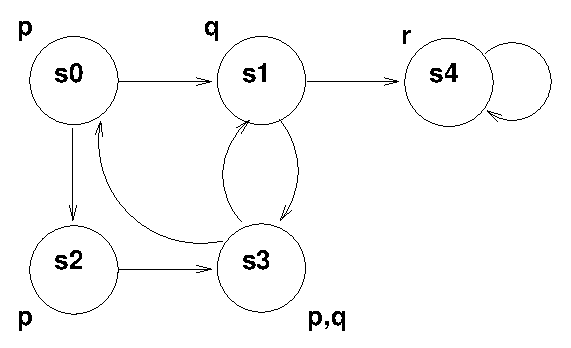
\includegraphics[scale=0.6]{../temporal-logics/diag23.eps}
\center
\caption{A sample Kripke structure} \label{fig2.1}
\end{figure}

\noindent
Fig~\ref{fig2.1} shows a Kripke structure consisting of 5 states. 
The nodes of Fig~\ref{fig2.1} are labeled by the atomic propositions
that are true at
that state. We shall use this toy example to demonstrate the meaning of
various temporal properties.

\noindent
To convey the semantics of the LTL operators, we will first
introduce the notion of a {\em run} (alternatively, a {\em path} or a
{\em trace}) of the Kripke structure $J$. A run, $\pi$, of $J$ 
is a sequence of states,
$\nu_0, \nu_1, \ldots$, where $\nu_0$ is the start of the run, and for
each $i$, $\nu_i$ represents a state in $S$, and $\tau$ contains a transition
from the state represented by $\nu_i$ to the state represented by $\nu_{i+1}$.
In other words, the run is a sequence of states representing a valid sequence
of state transitions of $J$. For example the run,
$\pi = s_0, s_1, s_3, s_1, s_4, \ldots$, is one run of the state machine shown
in Fig~\ref{fig2.1}. States of the machine may be revisited in the run -- 
for example we have $\nu_1 = \nu_3 = s_1$ in $\pi$. The run,
$\pi' = s_0, s_2, s_0, \ldots$, does not belong to this state machine, since
it has no transition from $s_2$ to $s_0$.

\noindent
Let $\pi = \nu_0, \nu_1, \ldots$ denote a run, and
$\pi^k = \nu_k, \nu_{k+1}, \ldots$ denote the part of $\pi$ starting from
$\nu_k$. We will use the notation $\pi \models f$ to denote that the property
$f$ holds on the run $\pi$. Given a run $\pi$, we will also use the notation
$\nu_k \models f$ to denote $\pi^k \models f$. In other words, a property is
said to be true at an intermediate state of the run iff the fragment of the 
run starting from that state satisfies the property.

\noindent
Let $f$ and $g$ be LTL formulas; $p$ is an atomic proposition and
$\pi = s_0, s_1, \ldots$ is a path in a Kripke Structure $K$. Then the
formal semantics of LTL may be defined as follows:
\begin{itemize}

\item $\pi \models p$ iff $p \in {\cal F} (s_0)$

\item $\pi \models \neg f$ iff $\pi \not\models f$

\item $\pi \models f \land g$ iff $\pi \models f$
        and $\pi \models g$

\item $\pi \models X\ f$ iff $\pi^1 \models f$

\item $\pi \models f\ U\ g$ iff $\exists j$,
        such that $\pi^j \models g$ and $\forall i, i<j$ we
        have $\pi^i \models f$

\end{itemize} 
\noindent
$Fg$ is a short-form for TRUE $U\ g$, and $Gf$ is a short-form for
$\neg F \neg f$. We say that the property $f$ holds
on a state machine, $J$, iff $f$ holds on all paths of the state machine
starting from its start state. 

\noindent
Let us see some sample LTL properties obtained by using one or more temporal
operators. We refer to Fig~\ref{fig2.1}.
\begin{itemize}

\item The property $p\ U\ q$ is true in the state machine, since all paths
	from $s_0$ satisfy this property.

\item The property $Fq$ is true in the state machine, but the property
	$GFq$ is not true. This is because we have the path, 
	$\pi = s_0, s_1, s_4, \ldots$, which does not satisfy $Fq$ from
	$s_4$ onwards.

\item The property $p\ U\ (q\ U\ r)$ is not true in the state machine, 
	because it may get trapped in the loop, $s_0, s_2, s_3, s_0$.

\end{itemize}
\noindent
Fig~\ref{fig2.2} shows some sample LTL properties and some runs
that satisfy these properties.

\begin{figure}[htb]
\centering
\includegraphics[scale=0.6]{../temporal-logics/diag24.pstex}
\center
\caption{Some sample LTL properties} \label{fig2.2}
\end{figure}

\subsection{Real time temporal logics} \label{sec2.1.3}
\noindent
Real time temporal operators are simple extensions of the basic
{\em untimed} temporal operators where we annotate the operator with a time
bound. The real time extensions of CTL~\cite{emerson:89} and 
LTL~\cite{alur:94} 
simply use these bounded operators (as well as the unbounded ones). 
\begin{description}

\item[The bounded Until operator: ] 
	The property $f U_{[a,b]} g$ is true on
	a run, $\pi = s_0, s_1, \ldots$, iff there exists a $k$, 
	$a \leq k \leq b$ such that $g$ is true at $s_k$ on $\pi$, and $f$
	is true on all preceding states, $s_0, \ldots, s_{k-1}$. Formally,
	\[ \pi\ \models\ f\ U_{[a,b]}\ g \mbox{ iff } \exists k,
	a \leq k \leq b, \nu_k\ \models\ g \mbox{ and } 
	\forall i, 0 \leq i < k \mbox{ we have } \nu_i\ \models\ f \]
	For example, the bounded LTL property $p\ U_{[1,3]}\ q$ is true at the state
	$s_0$ of Fig~\ref{fig2.1}. 

\item[The bounded Eventually operator: ] The property $F_{[a,b]} g$ is true
	on a run, $\pi = s_0, s_1, \ldots$, iff there exists a $k$,
	$a \leq k \leq b$ such that $g$ is true at $s_k$ on $\pi$.
	For example, the bounded LTL property $F_{[1,3]} q$ is true at the
	state $s_0$ of Fig~\ref{fig2.1}. The property $F_{[a,b]} g$ is
	equivalent to the bounded-until property, $true\ U_{[a,b]}\ g$. 

\item[The bounded Always operator: ] The property $G_{[a,b]} f$ is true
	on a run, $\pi = s_0, s_1, \ldots$, iff $f$ is true in every
	state in the sequence, $s_a, \ldots, s_b$. The bounded LTL property
	$G_{[0,1]} \neg r$ is true at $s_0$ since no run can reach $s_4$
	is less than 2 cycles.

\end{description}
\noindent
Real time operators are extremely useful in practice. Most design properties
have a well defined time bound, and must be satisfied within that time.
Since the real time operators deal with finite bounds, $a$ and $b$, they
can be expressed in terms of the $X$ operator. For example, the property
$F_{[2,4]} q$ can be rewritten as:
\[ {\tt F_{[2,4]}\ q\ =\ XX(q\ \lor\ Xq\ \lor\ XXq)} \]
and $p\ U_{[3,4]}\ q$ can be rewritten as:
\[ {\tt p\ U_{[3,4]}\ q\ =\ (p\ \land\ Xp\ \land\  XXp)\ \land\ 
	XXX(q\ \lor\ (p\ \land\ Xq))} \]
The first part of the property specifies that $p$ be must be true in the
present cycle and the next two cycles. The second part of the property
specifies that $q$ must be true in the third cycle, failing which, $p$
must be true in the third cycle and $q$ must be true in the fourth cycle.
Therefore, real time operators actually help us to succinctly express
properties that would require too many $X$ operators otherwise.

\subsection{Specification Languages used in Industry} \label{sec2.1.5}
The success of property verification in the industry depends to a large
extent on the evolution of language standards for property specification.
Currently {\em SystemVerilog Assertions} (SVA)~\cite{sva}, 
{\em Property Specification Language} (PSL)~\cite{psl},
{\em Open Verification Library} (OVL)~\cite{ovl}
are the three main contenders as languages for 
property specification. SVA is the natural choice for designers using
SystemVerilog. PSL is a good choice if one is working with VHDL, Verilog
or SystemC. OVL is a collection of libraries consisting of assertion 
templates in SVA/Verilog/VHDL.

\noindent
OVL, PSL and SVA were all developed initially under 
Accellera~\cite{accellera}. At this point, PSL has become
an IEEE standard (IEEE 1850 PSL), and SVA is part of the IEEE 1800 
SystemVerilog standard.  The complete syntax and semantics of SVA is given
in the SystemVerilog LRM. An overview of PSL is given in~\cite{perry:05}. 

\subsection{Formal Analysis of Specifications} 
The first major challenge faced by every verification engineer who uses
property verification is
to ascertain whether the specification itself is correct. Functional
correctness is very difficult to check since we do not have any formal
reference against which we may perform this verification. However it is
possible to check whether the specification is inherently consistent, or
whether there are contradictions within the specification itself.
Detecting inconsistencies in specifications is a non-trivial task, and
is therefore, an area of active research~\cite{pdgbook, prosyd}.
In this discussion, we briefly mention three popular consistency issues
in specification development, namely those of {\em satisfiability},
{\em realizability} and receptiveness. 

\subsection{LTL satisfiability} \label{sec2.2.1}
A system property over a set of variables is {\em satisfiable} if there
exists an assignment of values to the variables in each time step such that
the property is satisfied. Consider the LTL property $X\ p \land X\ \neg p$.
Clearly, this is unsatisfiable, while $X\ p \land F\ \neg p$ is
satisfiable. Consider the specification given in
Example~\ref{ex2.1}. The specification is satisfiable.

\noindent
LTL satisfiability has been well studied by researchers in the
academic community. In~\cite{vardi:86}, it is shown that LTL satisfiability
is PSPACE complete based on automata theoretic techniques.
LTL satisfiability is a part of most
existing model checking tools~\cite{forspec, vis, ifv, magellan}.

\subsection{LTL realizability} \label{sec2.2.2}
To explain the concepts of realizability and receptiveness, we need the
concept of an open system. Temporal logics like LTL and CTL were originally
defined for closed systems, that is, systems which are self contained and
have no external inputs. While this may be the case for a circuit as a 
whole, it is certainly not the case for the individual modules in the
circuit which will
typically receive inputs from the other modules. A module is an
{\em open system} (e.g. arbiter in Example~\ref{ex2.1}) whose behavior is a
function of the inputs it receives from its environment.

\noindent
The semantics of properties
for open systems may be viewed as a game between the module and its
environment, where the module decides the values of the output variables and
the environment decides the values of the input variables. A property
is {\em realizable} if a module is able to set the values of the
output variables in a way such that the property is satisfied for {\em all}
possible legal behaviors of the environment. However, this is not a
sufficient requirement. The system implementing the specification must not
be clairvoyant i.e. it must be able to assign its outputs without looking
at the future inputs. Consider the following example. 

\begin{example} \label{ex2.2}
{\em Let us examine the specification in Example~\ref{ex2.1}. The properties 
are:
{\tt
\begin{tabbing}
a\= aa\= aaa\= aaaa \= aaaaa \= aaaaaa\= aaaaaaa\= \kill
\>\>\>\>\>\> P1: G ($r_1$ $\Rightarrow$  X $g_1$ $\land$  XX $g_1$) \\
\>\>\>\> \>\>P2: G ($\neg r_1$ $\land$ $\neg r_2$ $\Rightarrow$  X $g_2$) \\
\>\>\>\> \>\>P3: G ($\neg g_1$ $\lor$ $\neg g_2$)
\end{tabbing}
}
\noindent
Let us consider the scenario, where $r_1$ is high at time $t$ and low at time
$t+1$, and $r_2$ is low at both time steps. The first property requires
$g_1$ to be high at time $t+2$, whereas the second property requires
$g_2$ to be high at time $t+2$ because both $r_1$ and $r_2$ are low at
$t+1$. The third property prevents both $g_1$ and $g_2$ to be asserted at
time $t+2$, leading us to a contradiction. The specification is therefore,
unrealizable, since there exists an assignment to the input signals
$r_1$ and $r_2$ for which no assignment to the output signals $g_1$ and
$g_2$ can satisfy the specification. The specification is however,
satisfiable, if we do not distinguish between the input and output
variables and treat the requests and grants in a similar fashion. In such
a case, an assignment to $r_1$, $r_2$ and $g_1, g_2$ is possible over
all time steps to satisfy the specification. 

\noindent
Before we proceed further, let us remove the inconsistency from our first
specification. The intent of the second property was to specify that $g_2$
is the default grant. Another way to specify the same intent is:
{\tt
\begin{tabbing}
a\= aa\= aaa\= aaaa \= aaaaa \= aaaaaa\= aaaaaaa\= \kill
\>\>\>\>\>\>\> G ($\neg g_1$ $\Rightarrow$  $g_2$)
\end{tabbing}
}
\noindent
This says that $g_2$ gets the grant whenever we are not committed to give the
grant to $g_1$. Henceforth we will use this property in place of the second
property in our specification. The overall specification of Example~\ref{ex2.1}
now becomes:

{\tt
\begin{tabbing}
a\= aa\= aaa\= aaaa \= aaaaa \= aaaaaa\= aaaaaaa\= \kill
\>\>\>\>\>\> P1: G ($r_1$ $\Rightarrow$  X $g_1$ $\land$  XX $g_1$) \\
\>\>\>\>\>\> P2: G ($\neg g_1$ $\Rightarrow$  $g_2$) \\
\>\>\>\> \>\>P3: G ($\neg g_1$ $\lor$ $\neg g_2$)
\end{tabbing}
}

\noindent
Let us see how this eliminates the problem. If $r_1$ is high at time $t$ and
low at time $t+1$, then the first property requires $g_1$ to be true at time
$t+2$. If $g_1$ is true, then the above property is vacuously satisfied
without requiring $g_2$ to be true, and hence there is no conflict.
} $\Box$
\end{example}

\noindent
The problem of realizability (also known as synthesizability) of LTL
specifications
has been well studied in the formal verification community. First identified
as Church's problem~\cite{church:63}, several methods have been proposed
for its solution~\cite{buchi:69, rab:72}. There are two (essentially
equivalent) approaches to solving the realizability problem. The first is by
reducing it to the emptiness problem of tree automata~\cite{rab:72}, and
the second, by reducing it to solving infinite-duration two-player
games~\cite{harding:05}.

\noindent
The problem of realizability of linear temporal logic specifications was
successfully solved in~\cite{pnueli:89}. This followed two previous
attempts~\cite{ce81, mw84} to synthesize programs from temporal 
specifications which reduced the synthesis problem to satisfiability,
ignoring the fact that the environment should be treated as an 
adversary.
As established in~\cite{vardi:86}, a LTL formula $\varphi$ is equivalent
to a B\"{u}chi automaton whose size is exponential in the length of
$\varphi$. The method for solving realizability as proposed
in~\cite{pnueli:89} for a given LTL specification
$\varphi$ starts by constructing a B\"{u}chi automaton for $\varphi$, which
is then determinized into a deterministic Rabin automaton~\cite{safra:88}. The
problem of realizability is finally solved by checking for emptiness of
the generated determinized Rabin automaton. The double translation
($\varphi$ to B\"{u}chi, B\"{u}chi to determinized Rabin) may cause a
complexity that is doubly exponential in $\varphi$. In fact, there is a lower
bound of $2^{O(nlogn)}$ for the number of states of a deterministic
automaton, given a B\"{u}chi automaton with n states~\cite{loding}.
The determinization construction used in~\cite{pnueli:89}
which converts a non-deterministic B\"{u}chi automaton to its
equivalent Rabin automaton is due to Safra~\cite{safra:88}. There is a
second construction, due to Muller and Schupp~\cite{muller}.
In~\cite{pnueli:89}, the authors further showed that the realizability 
problem for Linear Temporal Logic is 2-EXPTIME complete.

\subsubsection{Advances in realizability} \label{sec2.2.2.1}
The realizability problem inspired much research in this area for 
quite some time~\cite{ce81, harding:05,pnueli:89,prosyd}. The high 
complexity of the LTL realizability problem, as established 
in~\cite{pnueli:89} and the intricacy of the Safra's determinization 
construction inspired researchers to move
in two directions: (a) limiting the expressibility of the
specification to simpler automata or partial fragments of LTL~\cite{alur:04}
which have lower realizability checking complexity,
or (b) avoiding the intricacy of the determinization
construction~\cite{kupferman:05}. The second approach retains the
disadvantage of a higher complexity.

\noindent
In recent times, one of the most notable contributions in this direction
was achieved in~\cite{nir}, which shows that the complexity of the
realizability problem for LTL formulas 
belonging to the class of {\em generalized reactivity} of rank 1 (GR(1)),
is one exponential less than that of LTL by virtue of reduction to
Streett games. The class GR(1) covers a vast majority of
properties that appear in specifications of circuits.  The work
in~\cite{jobst} presents a tool called Anzu, that implements
a realizability checking procedure based on~\cite{nir}.

\subsection{LTL Receptiveness} \label{sec2.2.3}
\noindent
In practice, realizability is not an adequate requirement for the
consistency of a specification. Ideally, we expect a module to have
the freedom of choosing any valuation of its output variables that does not
refute the property. In some cases, a realizable specification may not
allow this freedom. Consider the following property for a module
having input $i$ and output $o$:
{\tt
\begin{tabbing}
a\= aa\= aaa\= aaaa \= aaaaa \= aaaaaa\= aaaaaaa\= \kill
\>\>\>\>\>\>\> G (o $\Rightarrow$  X i )
\end{tabbing}
}
\noindent
The property is realizable by any module that never asserts the output $o$.
The problem here is that the module needs to always assign $o=0$ because it
is unable to foresee the value of input $i$ in the next cycle. Therefore in
a given cycle, it does not have the freedom of assigning $o=1$ even though
that does not cause a refutation in that cycle. A specification that allows
the module to freely choose its outputs from those valuations that do not
cause an immediate refutation is called a {\em receptive} specification.
The notion of receptiveness was formalized by Dill in~\cite{dill:89}.

\subsection{Specification Development Styles} \label{sec2.1.6}
As more and more chip design companies attempt to integrate formal
property verification and dynamic property verification
into their pre-silicon validation flows, the main challenge that they
face is in the task of expressing the design intent correctly and
accurately in terms of formal properties. Incomplete specifications allow
bugs to escape detection, while inconsistent specifications lead to the
loss of validation effort, since the error lies in the specification itself.
This is aggravated by the fact that most modern formal specification
languages support an arsenal of features and constructs, an unrestricted
use of which is undesirable.
This has motivated much research in the academic and industry community
to standardize the process of formal specification development so that the
resultant specification is effective and easy to use. 

\noindent
Formal specification techniques typically differ by the particular
specification paradigm they rely on. In the sequel, we mention a few
of the popular specification development paradigms.

\begin{description}

\item [History-based Specification:] The principle here is to specify
    a system requirements by characterizing its maximal set of
    admissible histories. The properties of interest are specified
    by temporal logic assertions about system objects; such assertions
    involve operators referring to the past, current and future states.
    The assertions are interpreted over time structures. Time can
    be linear (LTL) or branching (CTL). Many of the temporal logics
    support the ability to express history using a {\em past}
    operator~\cite{ltlp}.

\item [State-based Specification:] Instead of characterizing the set
    of admissible histories, one may characterize the admissible system
    states at some arbitrary snapshot. The properties of interest are
    (a) invariants constraining the system objects at any snapshot, and
    (b) pre- and post-assertions constraining the application of
    system operations at any snapshot. Examples of this specification 
	style can be found in~\cite{Abr80, Abr96, gurevich, dill:00, dill:01}.

\item [Transition-based Specification:] Instead of characterizing
    system histories or states, one may characterize the required
    transitions from state to state. The properties of interest are
    specified by a set of transition functions; the transition
    function specifies for each input state and triggering condition,
    the set of allowable behaviors. Languages such as Statecharts~\cite{uml} 
	and PROMELA~\cite{spin} rely on this paradigm.

\item [Functional Specification:] The principle here is to specify the
    system requirements through a collection of mathematical functions.
    Languages such as OBJ~\cite{fut95}, HOL~\cite{gor93} or
    PVS~\cite{cro95} rely on this paradigm.

\item [Operational Specification:] System properties may be characterized by
    a collection of processes that can be executed by some more or
    less abstract machine. Early languages such as Paisley~\cite{zav82},
    Process Algebras~\cite{Hoa85} rely on this paradigm. 

\end{description}

\noindent
In recent times, some of the research on specification development 
paradigms has also been invested in 
restricting temporal logics to easy to use fragments for specifying a
system's functional properties. In~\cite{kmp98}, the authors have
proposed a methodology using logical constraints for environment
modeling for expressing bus protocols. In~\cite{dill:00,dill:01}, a
specification style was developed using the core subset of PCI as an
example. In this work, the authors used the concept of small
state machines (to be used as assertion monitors) and a set of
simple constraints for formal specification. However, the
constraints are simple propositional formulas with a time construct,
and therefore, can only capture a subset of the functional requirements.
In addition, the specification style has the restriction
that each constraint can only constrain the behavior of one agent.
Using this specification style, the work in~\cite{dill:01} has modeled
the formal requirements of the Intel Itanium Processor Bus
protocol and presents two debugging methods based on model
checking. In~\cite{gd00}, the authors have used this specification style to
formally verify a PCI driver implementation. Some of the other notable
research contributions in this area are reported in~\cite{cclw99, mhg98}.

\section{Formal Property Verification} \label{sec2.2}
\noindent
The FPV setup is shown in Figure~\ref{fig2.3}.
\begin{figure}[htb]
\centering
\psfrag{p1}{\small $G[r_1 \Rightarrow  Xg_1 \land  XXg_1 ]$}
\psfrag{p2}{\small $G[ \neg g_1 \Rightarrow  g_2 ]$}
\psfrag{p3}{\small $G[ \neg g_1 \lor \neg g_2 ]$}
\psfrag{p4}{\small $G[ \neg r_1 \land  X\neg r_1 \Rightarrow XX\neg g_1 ]$}
\includegraphics[scale=0.5]{../model-checking/fpv.pstex}
\center
\caption{Formal Property Verification Platform} \label{fig2.3}
\end{figure}
\noindent
At the heart of this approach, we have a
{\em model checking} tool. Popular model checking tools widely used in
the verification community today include VIS~\cite{vis}, NuSMV~\cite{nusmv},
Magellan~\cite{magellan}, IFV~\cite{ifv} and FormalPro~\cite{formalpro}.
A model checking algorithm has two main
inputs -- a formal property and a finite state machine representing the
implementation. The role of the algorithm is to search all possible paths
of the state machine for a path which refutes one or more properties. If one
exists, then the path trace is reported as the {\em counter-example}. Otherwise
the model checker asserts that the property holds on the implementation. 

\subsection{LTL Model Checking}
Given a model ${\cal M}$ described in some Hardware Description language (HDL) 
and an LTL specification ${\cal L}$, the model checking task is to 
determine whether the model ${\cal M}$ conforms to the semantics of ${\cal L}$. 
The traditional LTL model checking~\cite{lichtenstein:85} has the 
following steps:

\begin{itemize}
\item Extract the Kripke model from ${\cal M}$.

\item Build the tableau for $\lnot{\cal L}$ (call it 
						${\cal T}_{\lnot{\cal L}}$).

\item Compute the product of ${\cal M}$ and ${\cal T}_{\lnot{\cal L}}$.

\item Check the product machine for emptiness.

\end{itemize}

\noindent
If the product contains a run, then the model ${\cal M}$ has a run which 
satisfies $\lnot{\cal L}$ (and therefore, refutes ${\cal L}$). Hence the model 
checker reports the existence of a bug, and reports the run as the 
counter-example. If the product is {\em empty} (it contains no run), then it 
reports that ${\cal M}$ satisfies the property, ${\cal L}$.

\noindent
The complexity of model checking~\cite{schnoebelen:02} for 
linear temporal logic is PSPACE-complete. Given a transition 
system of size 	$n$ and a temporal logic formula of size $m$, 
the LTL model checking algorithm runs in O($n\times2^{O(m)}$) time.

\subsubsection{Model Extraction}
We will explain the generation of Kripke structure with the help of the example
arbiter discussed in Example~\ref{ex2.1}.
We have developed an implementation for our arbiter. The implementation and
the state machine of the implementation are shown in Figure~\ref{fig2.4}. 

\begin{figure}[htb]
\centering
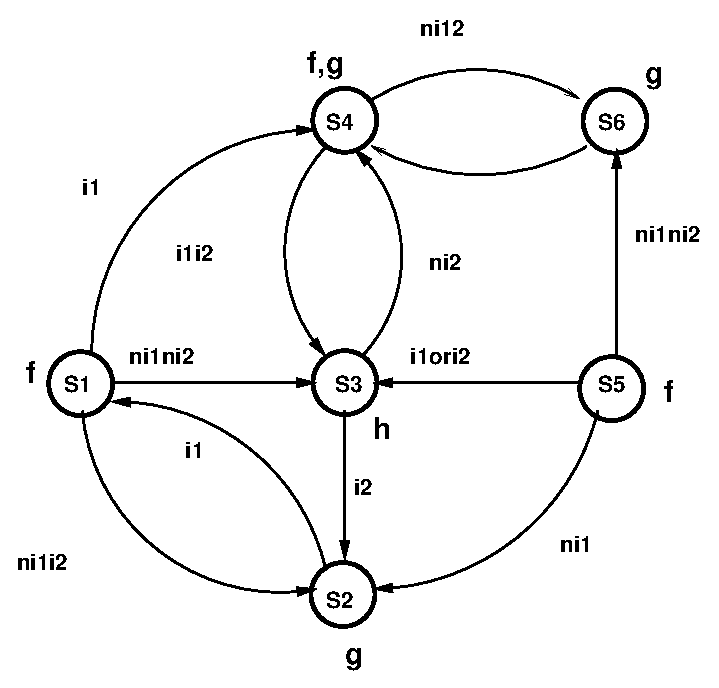
\includegraphics[scale=0.6]{../background/diag31.pstex}
\caption{Arbiter implementation and state machine} \label{fig2.4}
\end{figure}

\noindent
Since FPV must necessarily consider every possible run of the implementation,
FPV techniques require the state machine model of the implementation. 
Building the state machine model of the implementation is the single most
complex step of FPV, and accounts for the capacity limitations of existing
tools.

\begin{figure}[htb]
\centering
\includegraphics[scale=0.55]{../background/diag36.pstex}
\caption{State machine: Open and Closed forms} \label{fig2.5}
\end{figure}

\noindent
Figure~\ref{fig2.4} shows the state machine of our example arbiter.
Since the temporal properties do not distinguish between input and output
signals, we must transform this state machine into a {\em closed system}
-- where inputs are also part of the state definition. This is a simple
transformation, and the new state machine model is shown besides the original
one in Figure~\ref{fig2.5}. Each state of the original machine is now a cluster
of four states (shown as A, B, C, and D) -- the four states in a cluster
differ only in the input bits, that is, they have the same values for
$g_1$ and $g_2$. Each transition of the original machine is represented by
four transitions. Figure~\ref{fig2.5} shows these edges as
single edges leading to a block of states. For example, the transition from
state $01$ to state $00$ on input $00$ in the original state machine is now
represented by four non-deterministic transitions, namely $(0100, 0000)$, 
$(0100, 0001)$, $(0100, 0010)$ and $(0100, 0011)$. We show these four 
transitions in Figure~\ref{fig2.5} by a single edge from the state $0100$ 
to the 
block $A$, which consists of the four possible next states.
The new state machine is non-deterministic, simply because the next state
inputs are not known a priori.

\noindent
It can be seen that the closed system model of the arbiter represents the
Kripke structure for the arbiter which can be directly used by the model 
checking algorithm.

\subsubsection{Creating the tableau}
The tableau for a LTL property is 
a state machine, where each state bit is an {\em elementary subformula}
of the given property. Intuitively, these elementary subformulas are of two
types - Boolean formulas over the present state variables, and temporal
subformulas over future state variables.

\noindent
The set $EL(f)$ of elementary subformulas of $f$ is recursively defined as
follows:
\begin{itemize}
\item $EL(p) = \{p\}$ if $p$ is a signal or atomic proposition
\item $EL(\neg g) = EL(g)$
\item $EL(g \lor h) = EL(g)\ \cup\ EL(h)$
\item $EL(g \land h) = EL(g)\ \cup\ EL(h)$
\item $EL(Xg) = \{Xg\}\ \cup\ EL(g)$
\item $EL(g\ U\ h) =
        \{X[g\ U\ h]\}\ \cup\ EL(g)\ \cup\ EL(h)$
\end{itemize}
\noindent
Consider verifying the property $\psi$: $G[\ \neg g_1\ \Rightarrow \ g_2\ ]$
on the implementation of Fig~\ref{fig2.5}. The negation of $\psi$ is:
\[ \varphi: \qquad F[\ \neg g_1\ \land\ \neg g_2\ ] \] 
To verify $\psi$, we create the tableau for $\varphi$.
The set of elementary subformulas of $\varphi$
consists of  $g_1$, $g_2$, $X\varphi$. These three
elementary subformulas represent the state bits of the tableau, and thereby
yield $2^3 = 8$ states.

\noindent
The elementary subformulas are the ones whose truth dictates the state
of the property. For example, the property $\varphi$ above can be true at a
state in the following ways:
\begin{enumerate}

\item {\em Both $g_1$ and $g_2$ are false at that state}. The truth of
    $X\varphi$ is irrelevant here -- hence these cases are
    represented by two states of the tableau, namely:
    $\{\neg g_1, \neg g_2, X\varphi\}$ and
    $\{\neg g_1, \neg g_2, \neg X\varphi\}$.

\item {\em $g_1$ or $g_2$ is true at that state, and $X\varphi$ is
    also true at that state}. These cases are represented by three
    states of the tableau, namely: 
$\{g_1, g_2, X\varphi\}$, $\{g_1, \neg g_2, X\varphi\}$ and
    $\{\neg g_1, g_2, X\varphi\}$.
\end{enumerate}
\noindent
The second case needs more attention. $X\varphi$ is true at a state only
if $\varphi$ is true at the next state. Therefore, the tableau must have a
transition from a state satisfying $X\varphi$ to a state satisfying
$\varphi$. Similarly the tableau must have transitions from states
satisfying $X \neg \varphi$ to states satisfying $\neg \varphi$.
Fig~\ref{fig2.5a} shows the resulting tableau.

\begin{figure}[htb]
\psfrag{000}{\footnotesize $\neg g_1, \neg g_2, \neg X\varphi$}
\psfrag{001}{\footnotesize $\neg g_1, \neg g_2, X\varphi$}
\psfrag{010}{\footnotesize $\neg g_1, g_2, \neg X\varphi$}
\psfrag{011}{\footnotesize $\neg g_1, g_2, X\varphi$}
\psfrag{100}{\footnotesize $g_1, \neg g_2, \neg X\varphi$}
\psfrag{101}{\footnotesize $g_1, \neg g_2, X\varphi$}
\psfrag{110}{\footnotesize $g_1, g_2, \neg X\varphi$}
\psfrag{111}{\footnotesize $g_1, g_2, X\varphi$} 
\centering
\includegraphics[scale=0.5]{../model-checking/diag35.pstex}
\center
\caption{Tableau for $F[ \neg g_1\ \land\ \neg g_2 ]$}
\label{fig2.5a}
\end{figure}
\noindent
Let us refer to runs that satisfy $\varphi$ as {\em $\varphi$-satisfying runs}.
It is easy to see that every $\varphi$-satisfying run belongs to the tableau
and that these runs start from the states which are either labeled by
$\neg g_1 \land \neg g_2$, or are labeled by $X\varphi$. We shall refer to
these states (shown with double borders in Fig~\ref{fig2.5a}) as
{\em $\varphi$-satisfying states}. Every run that starts from the rest of the
states gets trapped between the three states $(\neg g_1, g_2, \neg X\varphi)$,
$(g_1, \neg g_2, \neg X\varphi)$, $(g_1, g_2, \neg X\varphi)$, and therefore
does not satisfy $\varphi$.

\noindent
Every run starting from a $\varphi$-satisfying state is not
a $\varphi$-satisfying run. Consider the runs that remain
forever within the three states, $(\neg g_1, g_2, X\varphi)$,
$(g_1, \neg g_2, X\varphi)$, and $(g_1, g_2, X\varphi)$. These runs do not 
eventually reach any state that satisfies $\neg g_1 \land \neg g_2$, and are
actually not $\varphi$-satisfying runs. Therefore only those runs are
$\varphi$-satisfying runs, that start from $\varphi$-satisfying states but
do not get trapped in $g_1 \lor g_2$ satisfying states. In general for any
property of the form, $f\ U\ g$, the run must not get trapped in
$\neg g$ labeled states. This is a typical instance of a {\em fairness
constraint}.

\noindent
As per our verification strategy, we seek a $\varphi$-satisfying run in the
implementation. This is done by computing the product of the tableau
with the implementation state machine and then checking whether
the product has any fair run starting from a $\varphi$-satisfying state.

\subsubsection{Computing the product}
The final step of our verification strategy is to compute the product of the 
state machine of the implementation with the tableau of the negation,
$\varphi$, of the original formal property, and check whether the product
contains a fair run starting from a $\varphi$-satisfying state of the
tableau.

\noindent
Fig~\ref{fig2.6} shows a fair run that is common between the state machine
model of the implementation shown in Fig~\ref{fig2.5} with the tableau shown
in Fig~\ref{fig2.5a}. This is one of many runs that may appear in the product
of the two machines -- each such run serves as a counter-example for the
property $\psi$ on the implementation of Figure~\ref{fig2.4}. 

\begin{figure}[htb]
\psfrag{000}{\footnotesize $\neg g_1, \neg g_2, \neg X\varphi$}
\psfrag{001}{\footnotesize $\neg g_1, \neg g_2, X\varphi$}
\psfrag{010}{\footnotesize $\neg g_1, g_2, \neg X\varphi$}
\psfrag{011}{\footnotesize $\neg g_1, g_2, X\varphi$}
\psfrag{100}{\footnotesize $g_1, \neg g_2, \neg X\varphi$}
\psfrag{101}{\footnotesize $g_1, \neg g_2, X\varphi$}
\psfrag{110}{\footnotesize $g_1, g_2, \neg X\varphi$}
\psfrag{111}{\footnotesize $g_1, g_2, X\varphi$}
\centering
\includegraphics[scale=0.5]{../model-checking/diag38.pstex}
\center
\caption{Tableau vs implementation} \label{fig2.6}
\end{figure} 

\subsection{State Space Explosion Problem}
The main bottleneck of FPV tools is in computing the product of 
the implementation and the tableau. It is interesting to note that the 
complexity of both CTL and LTL model
checking is linear in the size of the state machine of the implementation.
Intuitively this means that once we are able to build the state machine model
of an implementation, the task of checking the properties on the state machine
is not too complex. 

\noindent
However, FPV tools run into capacity issues while trying to build the state 
machine model of the implementation. An implementation consists of many 
concurrent components. When we have a formal property 
over the signals of one or more sequential components,
then FPV requires the {\em global state machine} obtained by computing the
product of the state machines of the components. This product leads to
state explosion.

\begin{figure}[htb]
\centering
\includegraphics[scale=0.6]{../model-checking/diag37.pstex}
\center
\caption{Product of state machines} \label{fig2.7}
\end{figure} 

\noindent
Fig~\ref{fig2.7} shows the product of two state machines, ${\cal M}_1$ and
${\cal M}_2$. In general if a module $M$ has $k$ component modules,
$M_1, \ldots, M_k$, having respectively $n_1, \ldots, n_k$ states, then
$M$ has at least $n_1 \times n_2 \times \ldots \times n_k$ states. This
figure grows alarmingly with increase in design complexity, and is popularly
known as {\em state explosion}.

\section{Advances in Model Checking} 
Various techniques have been developed and put into practice down the years 
to alleviate the state space explosion problem of model checking. 
The following sections 
describe some of the most important attempts in this direction.

\subsection{Symbolic Techniques}
Though the term {\em symbolic model checking} is popularly interpreted as 
BDD-based model checking, any model checking technique that works on a 
symbolic representation of the implementation can be called {\em symbolic} 
model checking. There are mainly three kinds of symbolic methodology 
found in the literature; namely {\em BDD-based model checking}, {\em SAT-based 
model checking}, and {\em ATPG-based model checking}.

\subsubsection{BDD-based Model Checking}
Binary Decision Diagrams (BDDs)~\cite{bryant:86} are compact canonical 
representations of Boolean functions. BDDs utilize self-similarity in 
the decision trees based on Shanon's expansion to give a more compact 
representation. Ken McMillan first proposed the model checking 
algorithms using BDD in his famous doctoral thesis~\cite{mcmillan:93}. The 
use of BDDs in model checking was instrumental in bringing the technology into 
practice. Experimental results showed that the BDD-based approaches were able 
to handle 10$^{20}$ states and beyond~\cite{burch:92} -- which was unthinkable 
with algorithms that work on explicit representations of the 
state space.

\noindent
BDD-based LTL model checking~\cite{clarke:94} is performed by 
transforming LTL model checking problem into a CTL model checking instance 
as follows:
\begin{enumerate}

\item The tableau ${\cal T}_{\lnot\varphi}$ is represented as a BDD, $Z$ (say, 
	$\varphi$ be the LTL formula of interest). Thus, $Z$ contains all valid 
	transitions present in the tableau.

\item Then the product of $Z$ with the BDD for the transition relation of
	the design under test (DUT) is computed. Let the BDD for the product be 
		${\cal P}$.

\item In the last step of the LTL model checking, the strategy is to
	check whether ${\cal P}$ is empty, that is, whether the product has any 
	fair path. This check
	is performed by verifying the CTL formula $EG[\ true\ ]$ on ${\cal P}$
	under fairness constraints~\cite{burch:90b,clarke:00}.

\end{enumerate}
 
\subsubsection{SAT-based Model Checking}
SAT is the traditional short form for the Boolean satisfiability problem. 
Given a Boolean formula $f$, the problem is to determine whether $f$ is 
satisfiable, that is, whether there exists any valuation of the variables 
in $f$, under which $f$ evaluates to $True$.
Verification methods based on the SAT problem have recently
emerged as a promising solution. Dramatic improvements in
SAT solver technology over the past decade have led to the
development of several powerful SAT solver 
tools~\cite{goldberg,zchaff,silva:99,quaffle}. 
Verification methods based on these tools have been shown
to push the envelope of functional verification in terms of
both capacity and efficiency, as reported in several academic
and industrial case 
studies~\cite{amla:03,amla:05,biere:99c}. 
This has fueled further interest and intense research activity in the area 
of SAT-based FPV.

\noindent
Bounded Model Checking based on SAT methods was introduced by Biere {\em et 
al.} in~\cite{biere:99a,biere:99,clarke:01} and is rapidly gaining popularity 
today as a complementary technique to BDD-based model checking. 
Given a temporal 
logic property $\varphi$ to be verified on a finite state transition system 
$M$, the essential idea is to search for counter-examples to $\varphi$ in the 
space of all executions of $M$ whose length is bounded by some finite 
integer $k$.

\noindent
The problem is formulated by constructing the following propositional formula:
	\[ f^k = I\ \land\ \bigwedge_{i=0}^{k-1} R_i\ \land\ (\lnot\varphi^k) \]
where $I$ is the characteristic function for the set of initial states of $M$, 
$R_i$ is the characteristic function of the transition relation of $M$ for 
time step $i$. Thus, the formula $I\ \land\ \bigwedge_{i=0}^{k-1} R_i$ 
precisely represents the set of all executions of $M$ of length $k$ or less, 
starting with an initial state. $\lnot\varphi^k$ is a formula representing 
the condition that $\varphi$ is violated by a bounded execution of $M$ of 
length $k$ or less. Hence, $f^k$ is satisfiable iff there exists an execution 
of $M$ of length $k$ or less that violates $\varphi$. $f^k$ is typically 
converted to CNF and solved by a conventional SAT solver.

\noindent
Due to the success of SAT solvers in bounded model checking, there has been 
growing interest in their use for {\em unbounded} model checking. Few of 
the recent works in this direction can be found in~\cite{kang:03,mcmillan:02}.

\subsubsection{ATPG-based Model Checking}
Recently there has been a growing interest in applying tools
for Automatic Test Pattern Generation (ATPG) of sequential
circuits to the model checking problem. ATPG tools for sequential
circuits are designed to search for input sequences to the given circuit that 
can test for the presence of a certain fault on the circuit outputs.
A sub-task in this process involves performing a search on
the space of input sequences of the sequential machine for an
input sequence that will excite a certain signal in the circuit
to logic 1 or 0. 

\noindent
Boppanna {\em et al.}~\cite{boppana:99} were the first to propose a sequential 
ATPG-based model checking technique. Further research on this technology can 
be found in~\cite{abraham:02,sheng:02}. The basic idea of this 
approach is as follows:
\begin{itemize}
\item 	Firstly, the temporal logic formula is translated into a monitor 
		automaton. The outputs from the DUT drive this automaton.
\item	Then a test network is added which produces ``1" iff the monitor 
		automaton reaches a {\em bad} state (where the property fails).
\item	Finally, sequential ATPG tools are employed to find out all the tests
		corresponding to a stuck-at-0 fault at the output of the test network.
		Clearly, the fault is {\em testable} (i.e., there exists an input 
		scenario which produces the complementary value of the fault at the 
		output) iff the temporal logic formula is {\em false} in the DUT.  
\end{itemize}

\subsection{State Space Minimization Techniques}
In this section, we describe several state space minimization techniques 
(developed to combat the state space explosion problem) which 
generate a minimized 
state transition graph corresponding to the DUT keeping the truth of all the 
temporal logic properties intact. All these techniques in essence make 
use of the structural information from the DUT and remove the portions of 
the design which are redundant in view of model checking (i.e., will not 
affect the truth of any property). The goal is to reduce the number of 
states considered in model checking, while preserving the correctness of 
the properties to be verified. 

\begin{figure}[htb]
\centering
\includegraphics[scale=0.6]{../model-checking/diag39.pstex}
\center
\caption{Cone of influence reduction with
    $G[\ r_1 \Rightarrow\  Xg_1\ \land\  XXg_1\ ]$} \label{fig2.8}
\end{figure}

\begin{figure}[htb]
\centering
\includegraphics[scale=0.6]{../model-checking/diag310.pstex}
\center
\caption{Reduced state machine, after COI} \label{fig2.9}
\end{figure}

\subsubsection{Cone-of-Influence Reduction}
The idea of cone-of-influence reductions~\cite{clarke:00} is to prune the 
circuit to remove all components that do not (directly or indirectly) 
influence the truth of the given property. 
For example, in order to verify the property:
{\tt
\begin{tabbing}
aaaa \= aaaa \= aaaa \= aaaaa\= aaaaaaa\= \kill
\>\>\>\> P1: \> G ($r_1$ $\Rightarrow$  X $g_1$ $\land$  XX $g_1$)
\end{tabbing}
}
\noindent
    on the implementation of Fig~\ref{fig2.5}, we observe that the
    logic for the output $g_2$ does not influence the truth of this
    property. We can therefore prune the circuit as shown in
    Fig~\ref{fig2.8}. The reduced state machine is much smaller,
    as shown in Fig~\ref{fig2.9}, which contains only those paths that
    are relevant to the final product. 

	\noindent
    Cone-of-influence reductions typically add a lot of value to an FPV
    tool, and these are an integral part of most FPV tools. Therefore if
    the designer can express the formal specification in terms of small
    properties over a few variables, then typically cone-of-influence
    reductions are able to effect sufficient pruning to avoid state
    explosion.

\subsubsection{Pruning using ``assume'' constraints.}
    Most property specification
    languages will allow the engineer to specify {\em assert} statements
    to describe the correctness requirements and {\em assume} constraints
    to indicate the assumptions about the inputs, under which the
    assertions are expected to hold.

	\noindent
    Intuitively, {\em assume constraints} can be used to prune the
    state machine of the implementation, since we need not consider
    those runs of the implementation that violate the assume constraints.
    In many cases, this can lead to significant reduction in the size 
	of the reduced state machine.

	\noindent
    Practitioners of FPV have also reported an exactly opposite experience
    at times with their FPV tools. They have observed that in some cases
    adding assume constraints into the specification have aggravated the
    capacity problem!

	\noindent
    This is {\em not} surprising. The state machine of the implementation
    may have to grow in size in order to incorporate a restriction which
    is temporal in nature. For example, consider the simple closed system
    state machine shown in Fig~\ref{fig2.9}. Suppose we add the
    assumption:
	{\tt
	\begin{tabbing}
	aaaa \= aaaa \= aaaa \= aaaaa\= aaaaaaa\= \kill
    \>\>\>\>\> G ($\neg r_1$ $\lor$ $\neg$ X $r_1$ $\lor$ $\neg$ XX $r_1$)
	\end{tabbing}
	}
	\noindent
    which says that {\em $r_1$ never comes in three consecutive cycles}.
    In order to incorporate this information into the state machine of
    Fig~\ref{fig2.9}, each state must {\em remember} the status of the
    request line in the previous cycle. This will lead to an
    increase in the number of state bits, and thereby the number of
    states of the state machine. 
	
\subsubsection{Equivalence relations for state space minimization}
    The state machine of an
    implementation may have more details than are required for verifying
    a given property. For example, consider the property P2 of
    Example~\ref{ex2.2}:
	{\tt
	\begin{tabbing}
	aaaa \= aaaa \= aaaa \= aaaaa\= aaaaaaa\= \kill
    \>\>\>\>\> P2: G ($\neg g_1$ $\Rightarrow$  $g_2$)
	\end{tabbing}
	}
	\noindent
    In order to verify this property we look for a path satisfying its
    negation:
	{\tt
    \begin{tabbing}
    aaaa \= aaaa \= aaaa \= aaaaa\= aaaaaaa\= \kill
    \>\>\>\>\> $\varphi$ = F ($\neg g_1$ $\land$ $\neg g_2$)
	\end{tabbing}
	}
	\noindent
    In order to check this property, we need to check whether any state
    satisfying $\psi = \neg g_1\ \land\ \neg g_2$, is reachable from the
    start state of the implementation. In other words, we may partition
    the states into two parts, those that satisfy $\psi$, and the rest.
    We want to determine whether it is possible to reach the first
    partition from the start state.

\begin{figure}[htb]
\psfrag{psi}{$\psi$}
\psfrag{npsi}{$\neg \psi$}
\centering 
\includegraphics[scale=0.5]{../model-checking/diag311.pstex}
\center
\caption{Equivalence with respect to $\psi = \neg g_1\ \land\ \neg g_2$}
\label{fig2.10}
\end{figure}

	\noindent
    We can minimize the state machine based on such partitions. For
    example, the reduced state machine after partitioning the state
    machine of Fig~\ref{fig2.5} around $\psi$ is shown in
    Fig~\ref{fig2.10}. The reduced state machine has only two states as
    compared to sixteen states of the original state machine.

	\noindent
    There are standard algorithms for minimizing a state machine based on
    a well defined equivalence relation. In the context of model checking,
    two of the most popular forms of equivalence are {\em bisimulation
    equivalence}~\cite{fisler:02} and {\em stuttering 
	equivalence}~\cite{clarke:00}. Stuttering equivalence 
    preserves the truth of untimed properties, such as $Fq$, where the 
    number of states on a path leading to a $q$-labeled state is not
    important -- these states may therefore be condensed into one state.
    On the other hand, in order to check a timed temporal property, such
    as, $F_{[3,9]}\ q$, we need to count the number of states on the path
    leading to a $q$-labeled state, and check whether this number is
    between $3$ and $9$. Therefore we cannot merge these states. However,
    two paths reaching the same $q$-labeled state in the same number of
    steps can be condensed into one path. Bisimulation equivalence is
    timing preserving.

\subsubsection{Counterexample Guided Abstraction Refinement}
Counterexample guided abstraction refinement~\cite{clarke:00b} 
is an iterative abstraction-refinement methodology in which an initial 
abstract model is generated by an automatic analysis of the control 
structures in the program to be verified. Abstract models may admit 
erroneous (or ``spurious") counter-examples. This methodology analyzes 
such counter-examples and automatically refines the abstract model 
correspondingly.

\noindent
The initial abstract model is constructed by using the {\em existential 
abstraction} techniques proposed in~\cite{clarke:00b}.
Then, a traditional model checker is used to determine whether the 
properties to be checked hold in the abstract model. If the answer is yes,
then the concrete model also satisfies the property. If the answer is no, 
then the model checker generates a counter-example. Since the abstract model 
has more behaviors than the concrete one, the abstract counter-example might 
not be valid. Such abstraction techniques are also known as false negative
techniques. When the model checker produces a counter-example, it is checked 
for validity. If the counter-example is found to be spurious, then the 
shortest prefix of the abstract counter-example that does not correspond 
to an actual trace in concrete model, is identified. The last abstract 
state in this prefix is split into less abstract states so that the spurious 
counter-example is eliminated. Thus a more refined abstraction function is 
obtained. There may be many ways of splitting the abstract state; each 
determines a different refinement of the abstraction function. It is desirable 
to obtain the coarsest refinement which eliminates the counter-example because 
this corresponds to the smallest abstract model that is suitable for 
verification.

\subsubsection{SAT-based Abstraction Refinement}
This is indeed a special case of the previous methodology where SAT solvers 
are used in counter-example guided abstraction refinement technique. One of 
the first attempts to use SAT solvers for counter-example guided abstraction 
refinement was described by Clarke {\em et al.}~\cite{clarke:02}. In their 
approach, the SAT solver is used to check whether a counter-example trace 
found during model checking of an abstract model is spurious or not, by 
effectively checking its satisfiability on the concrete design. If it is 
spurious, ILP (integer linear programming) and machine learning techniques 
are used to perform the refinement. In a subsequent effort~\cite{chauhan:02}, 
they used SAT-based techniques for performing this refinement as well.

\noindent
Another method for counter-example guided abstraction refinement using 
SAT solver has been proposed in~\cite{li:03,wang:03}. They use BDDs to 
represent multiple abstract counter-examples, which are checked for 
satisfiability on the concrete design using a SAT solver interfaced with 
BDD constraints~\cite{gupta:03}. Rather than refining each counter-example 
individually, they propose a game-theoretic refinement procedure, that 
attempts to exclude multiple spurious counter-examples simultaneously.

\subsubsection{Partial Order Reduction}
In asynchronous systems, interleaving of independent concurrent
events are equivalent, and only a representative interleaving needs to be 
explored to verify local properties. 
Partial order methods~\cite{godefroid:94,peled:93}
exploit this redundancy and visit only a subset of the reachable states.

\noindent
The method consists of constructing a reduced state graph. The full state 
graph, which may be too large to fit in memory, is never constructed. The 
behaviors of the reduced graph are a subset of the behaviors of the full 
state graph. The justification of reduction method shows that the behaviors 
that are not present do not add any information. More precisely, it is 
possible to define an equivalence relation among behaviors such that the 
checked property can not distinguish between equivalent behaviors. If a 
behavior is not present in the reduced state graph, then an equivalent 
behavior must be included. Hence, such methods are sometimes also called as 
{\em model checking using representatives}.

\noindent
Putting concurrent events in various possible orderings is a potential 
cause of state explosion problem in asynchronous systems. To see this, let 
us consider $n$ transitions that can be executed concurrently. In this case, 
there are $n!$ different orderings and 2$^n$ different states. If the 
specification does not distinguish between these sequences, it is clearly 
sufficient to consider only one sequence, with $n+1$ states. The partial 
order reduction is based on the {\em dependency relation} that exists 
between  the transitions of a system. Several algorithms have been proposed 
for this reduction technique. They differ in their approach to find the 
reduced state graph but follow the same partial order semantics. 
% as described 
%in~\cite{maz:89}. The reduction is performed by modifying the standard DFS 
%(Depth First Search)~\cite{cormen:90} algorithm to construct the reduced state 
%graph. The reduction can be applied {\em on-the-fly} while doing the model 
%checking~\cite{peled:94}. DFS can also be replaced by BFS (Breadth 
%First Search)~\cite{cormen:90} and combined with symbolic model 
%checking~\cite{alur:97,kurshan:98}.

\subsection{Modular Validation}
In view of the capacity limitations of model checking on large systems, the
verification perspective has shifted from a system level one to a module-level
one~\cite{kupferman:96}. The new methodology is popularly called 
modular validation. One of the
notable approaches to modular validation involves assume-guarantee based
compositional reasoning, where the system level verification task is
decomposed to a set of module level validation tasks.
Methods for {\em assume-guarantee} reasoning for open system verification
have been extensively studied for nearly three decades. {\em Assume-Guarantee}
reasoning was introduced by Chandy and Misra~\cite{chandy:81} and
Jones~\cite{jones} for analyzing safety properties. These methods were
extended to some progress properties in the following decade~\cite{panda}.
More recently, Abadi and Lamport~\cite{abadi:95} and Mcmillan~\cite{mcmillan}
extended the methods to temporal liveness properties. Several other
approaches to assume-guarantee reasoning have been proposed
in~\cite{kurshan:94,roever,stark}.

\noindent
The basic motivation behind assume-guarantee based compositional reasoning for
large systems is to ameliorate the state space explosion problem by
systematically decomposing the model checking task into smaller, more
tractable subtasks. There are two popular approaches towards assume-guarantee
reasoning for verification of modules, and most of the remaining are
derivatives of these. The first approach defines an interface
process (an interface of a module consists of its input-output behavior)
and verifies a module in isolation by composing the module
behavior with its interface. The interface process mimics the behavior of the
environment of the module and thus the desired verification task is
accomplished. In a second approach, for each module, the original
specification is partitioned into the assume and the guarantee
and the module is checked to determine whether it satisfies the guarantee
in presence of the assumptions, and a composition rule is defined to compose
the verification tasks for each module to reason about the entire system.
These two ideas rest behind most of the approaches in assume-guarantee
reasoning~\cite{abadi:95,chandy:81,henzinger:00,jones,josko,panda,roever,stark}.

\noindent
However, both the above approaches are non-trivial. The
construction of the interface process is difficult in the former approach while
the latter approach is non-trivial due to the inherent intricacy involved
in assume-guarantee separation of the specification. 
Furthermore, as shown by Namjoshi and Trefler~\cite{namjoshi},
most of the existing methods for compositional reasoning based on
the assume-guarantee paradigm can be hard to apply, for a number of
reasons. Firstly, they are often bound to a particular syntax for
describing processes, and particular notions of behavior and composition.
Thus, it is not clear whether a reasoning pattern devised for one such
choice also applies to another. Another key factor is that several
methods are known to be incomplete~\cite{namjoshi}, usually for liveness
properties of simple programs. The completeness failure can usually be traced
back to restrictions placed to avoid unsound, semantically circular
reasoning with assumptions and guarantees. An incomplete procedure is
an impediment in practice. Lastly, safety and liveness properties are
handled differently by most methods.

\noindent
To overcome the limitations of assume-guarantee methods in practice, several
advances have been made and an arsenal of assume-guarantee composition rules
have been formulated. Namjoshi and Trefler~\cite{namjoshi} have proposed a
complete method for model checking of linear time temporal properties. 
In~\cite{amla1}, Amla, Emerson, Namjoshi and Trefler have presented a
new rule for assume-guarantee reasoning which generalizes several earlier rules
~\cite{abadi:95,jones,namjoshi,pnueli:84} by removing the sources of
incompleteness in some of these rules, by using processes instead of temporal
logic formulas as specification and allowing more general forms of process
definition and composition. Further, they have shown that timing diagrams
have a natural decomposition into assume-guarantee pairs, and liveness
restrictions that can be checked efficiently and presented a tool which
carries out the reasoning in a fully automatic manner. The same group of
authors have presented a similar work on regular timing diagrams
in~\cite{amla2,amla3}. In~\cite{amla4}, they have  proposed
an abstract framework for process composition, formulated an assume-guarantee
method, and showed that it is sound and complete. In another
work~\cite{amla5}, they have proposed a new framework, called Modular Timing
Diagrams (MTD) for specifying the universal properties about causality and
timing of events in an asynchronous system along with a method for
automatically generating an assume-guarantee partitioning of an MTD.
In~\cite{schloer}, Schl$\ddot{o}$r has proposed a visual specification
formalism called Symbolic Timing Diagram (STD) and its extension called
Linear Symbolic Timing Diagram (LSTD), which can be used to verify models of
reactive systems. They have also developed a methodology for open system 
verification based on compositional reasoning of STDs.
In another approach, Thiagarajan and Henriksen~\cite{dltl}
have proposed a new logic
called Dynamic linear time temporal logic (DLTL) by extending LTL along
two dimensions. They have shown that their logic has a natural semantics in
terms of runs of a distributed program consisting of a finite set of
sequential programs that communicate with each other by performing
common actions together. 

\section{Dynamic Property Verification} \label{sec2.4}
The DPV setup is shown in Figure~\ref{fig2.11}.
There are two key features of DPV which explain the remarkable growth
in the penetration of this approach. Firstly, it is built over the
traditional simulation framework and requires nominal additional effort
from the verification engineer. Secondly, it does not have any major capacity
concerns, since the verification is done over the simulation run.
The VCS~\cite{vcs} tool from Synopsys has DPV capabilities, where
the properties are to be described in System Verilog Assertion~\cite{sva}
and the DUT is described in a Hardware Description Language (Verilog,
VHDL or System Verilog).

\begin{figure}[htb]
\centering
\includegraphics[scale=0.45]{../intro/diag2.pstex}
\center
\caption{DPV Platform} \label{fig2.11}
\end{figure}

\subsection{DPV Basics}
DPV is a simulation-based approach, where the properties are checked over 
a simulation run.  As in simulation, we write a test bench to drive inputs 
into the implementation. 
At the heart of DPV is the concept of monitoring properties over 
simulation runs. Before we present the concept of dynamic monitoring, 
we present two useful definitions below:

\begin{definition} {\bf [X-pushed formula: ]}\\
A formula is said to be X-pushed if all the X operators in the formula are
pushed as far as possible to the left.
\end{definition}

\begin{definition} {\bf [X-guarded formula: ]}\\
A formula is said to be X-guarded if the corresponding X-pushed formula
starts with an X operator whose scope covers the whole formula.
\end{definition}

\begin{example}
{\em
Let us consider the temporal property
{\tt
\begin{tabbing}
aaaa \= aaaa \= aaaa \= aaaaa\= aaaaaaa\= \kill
\>\>\>\>\> ${\cal P}$ = ((X p) U (XX q)) $\land$ (XF r)
\end{tabbing}
}
\noindent
The X-pushed form of $\cal P$ is:
{\tt
\begin{tabbing}
aaaa \= aaaa \= aaaa \= aaaaa\= aaaaaaa\= \kill
\>\>\>\>\> ${\cal P}_X$ = X ((p U (X q)) $\land$ (F r))
\end{tabbing}
}
\noindent
Now ${\cal P}$ is a X-guarded formula as the corresponding X-pushed
formula  ${\cal P}_{X}$ starts with a X operator whose scope covers the
 whole formula.
}$\Box$
\end{example}

\noindent
The task of monitoring the truth of a given LTL property along a simulation
run works as follows. If we are required to check a LTL property, $\varphi$,
from a given time step, $t$, we rewrite the LTL property into a set of
propositions over the signal values at time $t$ and a set of X-guarded LTL
properties over the run starting from time $t+1$. The rewriting rules are
standard, and are as follows:
\begin{eqnarray*}
f\ U\ g & = & g\ \lor\ (f\ \land\ X(f\ U\ g)) \\
Fg & = & g\ \lor\ XFg \\
Gf & = & f\ \land\ XGf
\end{eqnarray*}
\noindent
At the end of the simulation
step, we substitute the current signal values in the right hand side (RHS)
to determine the temporal property that needs to be checked in the next cycle.
We proceed to the next simulation step with this new property.

\begin{example}
{\em
Suppose the designer wants to forbid the satisfaction of the property:
\[ \varphi\ =\ p\ U\ (q\ U\ r) \]
\noindent
In other words, the correctness property is $\neg \varphi$, and in order to
verify it we search for a match of $\varphi$. We start the simulation with
the property $\varphi$ at $t=0$. Let us assume that the initial signal values
are $p=1, q=0, r=0$. At $t=0$ we rewrite $\varphi$ as:
\begin{eqnarray*}
\varphi & = & (q\ U\ r)\ \lor\ (p\ \land\ X(p\ U\ (q\ U\ r))) \\
& = & (r\ \lor\ (q\ \land\ X(q\ U\ r)))\ \lor\
        (p\ \land\ X(p\ U\ (q\ U\ r)))
\end{eqnarray*}
\noindent 
Substituting the initial values, $p=1, q=0, r=0$, we get:
\begin{eqnarray*}
X(p\ U\ (q\ U\ r)) & = & X \varphi
\end{eqnarray*}
\noindent
We proceed to the next simulation step. Suppose the signal valuations in the
next cycle are $p=0, q=1, r=0$. Again we rewrite $\varphi$ as above and
substitute the present state signal values. This time the resulting
property for the next cycle is:
\begin{eqnarray*}
\psi & = & q\ U\ r
\end{eqnarray*}
\noindent
In the next cycle, we will rewrite $\psi$ using the same rules:
\begin{eqnarray*}
\psi & = & r\ \lor\ (q\ \land\ X(q\ U\ r))
\end{eqnarray*}
\noindent 
Suppose simulation now returns $p=1, q=0, r=1$. Substituting this in the
above formula yields true. Hence we have a match for $\varphi$, which 
in turn is a refutation of our correctness property.
} $\Box$
\end{example}

\noindent
As another example, let us consider the arbiter of Example~\ref{ex2.1}
and its implementation in Figure~\ref{fig2.4}.

\begin{example} \label{ex2.3}
{\em Consider the property P1, that is:
\[ {\tt P1: \qquad G[\ r_1 \Rightarrow\  Xg_1\ \land\  XXg_1\ ]}  \]
We will first create the negation of P1 - let us call it $\varphi$:
\[{\tt \varphi\ =\ F(\ r_1\ \land\ (X \neg g_1\ \lor\ XX \neg g_1))} \]
At the start state, we need to check $\varphi$ -- we will therefore rewrite
it as: 
\[{\tt \varphi\ =\ (r_1\ \land\ (X \neg g_1\ \lor\ XX \neg g_1))\ 
	\lor\ X\varphi} \]
As long as the test bench does not assert $r_1$, the first term in this
formula will be false.

\noindent
When the test bench drives $r_1$ (say at time $t$), the new property will be:
\[ {\tt (X \neg g_1\ \lor\ XX \neg g_1)\ \lor\ X\varphi} \]
which is obtained by substituting $r_1 = 1$ in $\varphi$. Therefore, in the
next cycle, $t+1$, we look for:
\begin{eqnarray*}
\psi & = & \neg g_1\ \lor\ X \neg g_1\ \lor\ \varphi \\
     & = & \neg g_1\ \lor\ X \neg g_1\ \lor\
    ((r_1\ \land\ (X \neg g_1\ \lor\ XX \neg g_1))\ \lor\ X\varphi)
\end{eqnarray*}
\noindent
In response to the stimulus $r_1 = 1$, the arbiter implementation of
Fig~\ref{fig2.4} will assert $g_1$ at time $t+1$. Suppose that the test 
bench drives $r_1 = r_2 = 0$ at time $t+1$. Substituting this
information in $\psi$ gives us:
\[ {\tt X \neg g_1\ \lor\ X\varphi} \]
which yields the property:
\[ {\tt \eta\ =\ \neg g_1\ \lor\ \varphi} \]
for $t+2$. In response to the stimulus
$r_1 = r_2 = 0$ at time $t+1$, the arbiter will assert $g_1 = 0$ at time
$t+2$. This will satisfy $\eta$ and will indicate a match of $\varphi$.
Since $\varphi$ is the negation of P1, we have found a refutation of P1,
and uncovered a bug!} $\Box$
\end{example} 

\subsection{DPV Limitations}
\noindent
Our success in finding the bug of Example~\ref{ex2.3} relies on the
assumption that the test bench will drive $r_1 = 1$ at some time $t$ and
then drive $r_1 = r_2 = 0$ in the next cycle, $t+1$. If the test bench
never drives such a sequence of inputs, the bug will escape detection.

\noindent
The example brings out one of the major challenges in property verification.
In the DPV approach, we write a test bench to drive inputs
into the implementation. The complexity of this task grows rapidly with the
complexity of the design. This is because the environment of a module is
typically constrained by the behavior of the other modules in the design
and by the protocol used for their communication.  

\noindent
For example, let us consider the task of verifying a master interface in
the ARM AMBA AHB~\cite{ahb} protocol. The Bus architecture is 
shown in Fig~\ref{fig2.12}.
The Bus supports several different types of transfers -- read and write
transfers, single and burst transfers, incremental bursts and bounded bursts,
locked transfers. It also supports split transfers and retry responses. It
supports both types of endianness. Since the master can initiate and
participate in these different types of transfers, a test plan for the master
must cover many different cases. In order to drive meaningful inputs into the
module, a test environment for the master must correctly mimic the behavior
of the other components such as the slave devices, the Bus arbiter, the bridge
to the APB Bus, and other contending master devices. The validation engineer
must be aware of the protocol followed by the other components while
developing a test for a given master interface, which is a non-trivial task.

\begin{figure}[htb] 
\centering
\includegraphics[scale=0.6]{../testgen/diag71.pstex}
\center
\caption{An Arm AMBA Architecture} \label{fig2.12}
\end{figure}

\noindent
As the design complexity increases, we face two problems, namely (a) the
number of directed tests required to cover all the interesting behaviors
grow alarmingly, and (b) the task of writing each directed test becomes
more complex, thereby requiring more time from the validation engineer. 

\noindent
In view of its inherent dependence on the availability of good test 
vectors, the main limitation of DPV is that the coverage of
the corner cases for which a property was written depends entirely on the test
generator's ability to reach those corner cases by driving the appropriate
inputs into the DUT. If none of these corner cases are reached during
simulation, then the property remains {\em unutilized}, since we have not
checked whether the DUT satisfies the property in those corner cases. 

\section{Advances in DPV}
To address the issue of effective test generation for ensuring higher 
coverage in a simulation-based validation 
framework, several research efforts have been investigated in the 
past few years. Below, we mention some of these.

\subsection{Constrained Random Test Generation}
\noindent
In recent times, 
the industry appears to be moving towards simulation frameworks that employ
a coverage driven random test generation approach, as opposed to the
traditional approach of writing directed tests. 

\noindent
The intuitive motivation behind this approach is 
to use randomization at the real {\em choice points}
of the environment. For example, there are several choice points for the
test environment of a AMBA AHB slave interface. We may randomly choose the
transfer type (read/write, single/burst etc) and the master which initiates
the transfer. Once we have chosen the transfer type and the
master, the test bench initiates the transfer by imitating the transfer
request from the master in a protocol compliant manner. The length of the
transfer, the values of the address and data lines are the choice points
during the transfer. None of these choices are unconstrained. For example,
to choose the given slave in a memory mapped system, the values of the
address lines have to be constrained so that the address lies in the map
of the device.

\noindent
Monitoring the coverage is a very important component of the constrained
random verification approach. Since the tests are generated randomly, we
must know which behaviors have been covered. Recent test bench languages
such as the test bench language of SystemVerilog enables a validation
engineer to specify the coverage goal, to bias the random 
choice at choice points by associating weights with the choices and 
to monitor the status of the coverage.

\subsection{Layered Verification Methodologies} \label{layered}
In the last few years, several EDA companies are promoting a structured
hierarchical methodology for developing the simulation test environment
for complex digital designs. These include the {\em e-Reuse Methodology} 
(eRM)~\cite{erm} of Verisity, the {\em Reference Verification 
Methodology} (RVM) of Synopsys~\cite{rvm},
and {\em Verification Methodology} (VMM)~\cite{bergeron:05} of ARM and Synopsys.
The focus of these methodologies is in enabling the validation engineer to
develop a set of functional models for the components of a large design
and then using these models in a constrained random test generation
environment. 

\noindent
Recent design and verification languages such as SystemVerilog and $e$ support
the style of verification suggested by these methodologies. SystemVerilog,
for example, is a combination of a design language (Verilog) and a test bench
language.
The test bench language supports a large set of powerful constructs
that facilitate the development of behavioral models for the components of a
large design. For example, the SystemVerilog test bench language supports
fork-join constructs, synchronization constructs such as semaphores,
communication constructs such as channels, and a fully object oriented
design style.

\noindent
{\em The behavioral models help in building a randomized test
environment.} The test bench language supports features that enable the
validation engineer to call a randomizer to choose the values of signals
under specified constraints. The models of the components use this feature
at each choice point. The test bench instantiates those models that
constitute the environment of the DUT and handles the high-level choices
(such as the choice of the transaction type) randomly. The models randomly
generate their responses in a protocol compliant manner and this guarantees
that the inputs driven into the DUT are also protocol compliant. 

\begin{figure}[htb]
\centering
\includegraphics[scale=0.6]{../testgen/diag72.pstex}
\center
\caption{A Layered Test Architecture} \label{fig2.13}
\end{figure}

\noindent
These ideas have been integrated into a systematic layered approach for
creating a test environment. The typical layers in a RVM or VMM compliant
test architecture are shown in Fig~\ref{fig2.13}. We briefly outline the
meaning of these layers in the context of a Bus protocol (say, AMBA AHB).
\begin{itemize}

\item {\em Signal Layer.}
    The sensitization of the DUT takes place in this
    layer. The interfaces of the DUT with the test bench and the monitor
    are defined at this layer.

\item {\em Command Layer.} 
    This layer drives the unit level transactions
    through the DUT (using the signal layer). For example, typical
    transfer types in AMBA AHB includes {\em idle, read, write,
    burst-read}, and {\em burst-write}. The command layer needs to be
    aware of the Bus protocol, and must drive the transactions in a
    protocol compliant manner. This task becomes significantly easier
    when the models of the components of the architecture are used. For
    example, when we need to drive a write transfer to a slave DUT, it
    makes our task significantly easier if we have the behavioral model
    of a protocol compliant master to drive the transfer.

\item {\em Functional Layer.} 
    This layer creates sequences of transactions,
    and then requests the command layer to drive each transaction in the
    appropriate sequence. Examples include, {\em read followed by
    burst-write}, and {\em burst-write followed by idle}.

\item {\em Scenario Layer.} 
    Architectural scenarios are generated at this 
	layer. For example, consider the handling of an interrupt. An
    interrupt can happen in many ways, and can be handled in many ways
    -- each of these cases is a potential test scenario. Other examples
    include DMA, cache flush, etc. Each scenario consists of a sequence
    of transactions, which is handled by the functional layer.

\item {\em Test Layer.} 
    The test cases are specified at the highest level
    of abstraction in this layer. The contents of this layer is mostly
    application specific.	

\end{itemize}

\noindent
Recent test bench languages such as SystemVerilog provide a communication
primitive called {\em channels} for facilitating the communication between
the layers of the test bench. The validation engineer is expected to model
all communications between the layers using channels.

\noindent
Assertions fit into this architecture everywhere. 
At the command layer, we need assertions to verify
whether the transactions are compliant with the Bus protocol. At 
the functional
layer, we need assertions to verify whether the pipelining between successive
transfers is being done correctly. At the higher layers, we need assertions
to verify whether in each scenario, the application specific properties
relevant to that scenario are being satisfied. In Fig~\ref{fig2.13}, the
assertions are shown between the command layer and the functional layer
because the assertion IP for the AMBA protocol (which is application
independent) resides in these layers. Application specific assertions can
off course be specified and used at the higher layers of the architecture.

\subsubsection{The benefits}
Writing the behavioral models for the components of a large design (and
validating them) requires a significant quantum of time. However, once the
models are complete, we are in an advantageous position. In order to verify a
given DUT, we can quickly construct a test bench by instantiating the models
that constitute the environment of the DUT. After this, we begin the
simulation and no user intervention is required. Since the test bench
generates tests randomly, successive iterations of the test bench
automatically sensitizes different scenarios and automatically reaches
different coverage points. As a result, the test bench covers a
large number of coverage points very quickly.

\begin{figure}[htb]
\centering
\includegraphics[scale=0.6]{../testgen/diag73.pstex}
\center
\caption{Coverage: Directed versus Randomized} \label{fig2.14}
\end{figure}

\noindent
Fig~\ref{fig2.14} shows a typical comparison of the coverage times between the
traditional approach of writing directed tests and the new approach of
constrained random test generation.
In the traditional approach, the coverage of behaviors starts right from the
beginning, since the simulation can begin as soon as the validation engineer
has developed a test. The slope of the curve depends on the manpower used
for writing the tests.

\noindent
In the constrained randomized approach, simulation starts only after the
behavioral models for the components of the environment have been completed.
Therefore, there is an initial period when no coverage is achieved -- this 
is the model building phase. The length of this phase depends on the manpower
used for developing the models. Once the models are complete and the simulation
starts, we see a rapid growth in the coverage. The slope of this curve
is dictated by the speed of the simulation and the effectiveness of the
randomization in reaching the different coverage points. Significantly,
{\em the slope of this curve is independent of the manpower used}.

\noindent
Typically the new approach {\em overtakes} the traditional approach in large
designs in terms of speed of coverage. However during the inception of this
approach in companies, validation teams are usually under tremendous
pressure in the model building phase since they do not have any coverage
to show.

\subsubsection{The limitations} 
The probability of a specific scenario being generated randomly 
is the product of the
probabilities of making the right choices at the choice points that lead to
the given scenario. Therefore, if a corner case can be reached through a
very special sequence of choices, and the probability of picking the right
choice is low in each step, then the probability of coverage of the corner
case may become quite low.

\noindent
Let us consider an example. Let us say that a master device makes a Bus request
10\% of the time (that is, with a probability of $0.1$). The Bus protocol
exhibits some special behavior when none of the masters are requesting --
it parks the grant on a default master. It also exhibits some special
behavior when {\em all} the masters are requesting -- it sends a hold signal
to the bridge connecting to the low performance Bus. We want to cover both
scenarios in a system of 5 masters.

\noindent
Our choice points here are the requesting status of the masters.
\begin{enumerate}

\item For the first case, the probability that a master is not requesting
    is $0.9$. Hence the probability that none of the masters are 
	requesting is $(0.9)^5$. With this probability,
    it is quite likely that this corner case will be covered.

\item For the second case, the probability that a master is requesting is
    $0.1$, and hence the probability that all of them are requesting is
    $0.00001$, which is very small. With this probability, it is much
    less likely that this corner case will be covered, unless we run the
    simulation for a long time.

\end{enumerate}
\noindent
This is a standard problem in randomized testing -- we reach a lot of coverage
points very fast, but it takes a lot of time to cover the corner cases that
have low probability of occurrence. In other words, the simulation tends to
get trapped in the common behaviors and fails to sensitize some of the
interesting uncommon behaviors. 

\noindent
The most common approach to get around this problem is to write
directed tests for the special corner cases that were not covered by
randomized testing. While this seems to be the most logical thing to do, it
does take a significant amount of validation time, because the remaining
scenarios are difficult to conceive and finding the right tests to adequately
cover these cases is not straight forward. Recent research is attempting to
find automated solutions to the problem. 

\noindent
The intuitive idea being pursued by several researchers is to use the
coverage feedback dynamically to find the gap between the coverage goal
(that is, what needs to be covered) and the coverage status (that is,
what has been covered) and to {\em automatically guide the test generator
towards the gaps}. The idea seems to be applicable at all layers of the test
architecture, and at various levels of abstraction. 

\subsection{Enhancing Assertion Coverage in DPV}
\noindent
The main limitation of dynamic property verification is that the coverage of
the corner cases for which a property was written depends entirely on the test
generator's ability to reach those corner cases by driving the appropriate
inputs into the DUT. If none of these corner cases are reached during
simulation, then the property remains {\em unutilized}, since we have not
checked whether the DUT satisfies the property in those corner cases.

\noindent
An assertion is a concise specification of a set of corner
case behaviors. Therefore, we need to treat assertions as coverage points
and make sure that the simulation reaches those behaviors for which an
assertion has been written.

\noindent
One option for solving this problem is by writing directed tests
to cover the behaviors for which the property was written. There are at least 
two major criticisms of this approach:
\begin{enumerate}

\item The property encodes the behaviors for which it was written. Having
    to write the directed tests again to cover the same behaviors is
    (theoretically) repetition of information, which ideally (that is,
    given the right technology), should not be necessary.

\item A property can be {\em triggered} in complex ways. It is not easy for
    a validation engineer to visualize all types of scenarios in which
    the property may become relevant.

\end{enumerate}

\noindent
In recent times, several researchers have attempted to find an 
automated solution to this problem. We mention some of these efforts 
below.

\subsubsection{Assertion-guided test generation}
A broad span of research from early work on algebraic
specifications~\cite{gannon:81} to more recent work such as~\cite{stocks:96}
addresses the problem of relating tests to formal specifications.

\noindent
One of the main research directions on this topic is on the use of special
constructs for characterizing the input space. In~\cite{clarke:00a}, Clarke
{\em et. al.} have proposed a methodology which uses a statically-built BDD
to represent the entire input constraint logic. Shimizu
{\em et. al.}~\cite{shimizu:02} describe an approach in which the same formal
description is used for collecting coverage information and deriving simulation
inputs.  There have been many efforts based on constraint solving for test
generation as reported in~\cite{huang:02}.

\noindent
Offline monitoring for test generation is another notable approach.
In~\cite{tasiran:03}, Tasiran {\em et. al.} use the following approach.
Simulation steps are translated (offline) to protocol state transitions using
a refinement map and then verified against the specification using a model
checker. On the specification state space, the model checker collects coverage
information, which is used for future test generation. Another approach is
proposed in~\cite{gupta:02}, where the authors present a methodology for 
automatically determining the appropriate vector constraints, based on the
analysis of both the design and the property being checked.

\noindent
ATPG based techniques have been used in~\cite{abraham:02,boppana:99} for
automatic test generation. In these approaches, the formal properties are
synthesized as non-deterministic state machines and ATPG is targeted towards
faults representing a discrepancy between the implementation and the
state machine representing the specification.

\noindent
In {\em counterexample guided test generation}, the model checker is used as
an oracle to compute the expected outputs and the counterexamples it generates
are used as test sequences. The counterexamples contain both inputs and
expected values of outputs and so can automatically be converted to
test cases~\cite{ammann:98,gargantini:99}. In another work, Callahan,
Schneider, and Easterbrook have presented a methodology using the SPIN model
checker to generate tests that cover each block in a certain partitioning of
the input domain~\cite{callahan:96}. 

\section{Semi-Formal property verification} \label{sec2.3.5}
In recent times, there has been a rising trend towards the 
deployment of semi-formal techniques, where multiple 
verification techniques are applied in a way that they complement 
one another resulting in better verification performance, both in 
terms of design size and coverage. A major challenge in this area 
is to ensure that the techniques complement each other rather than 
subvert each other when working in tandem. An excellent survey of 
successful deployment of semi-formal verification approaches appears 
in~\cite{bhadra:07}. In this discussion, we mention a few of these 
which are related to our work. 

\noindent
In~\cite{ho, ho1}, the authors combined the use of scalar and
symbolic simulation together with BMC for improving automatic test
generation and unreachability analysis. The approach in~\cite{aagard}
uses theorem-proving techniques to coordinate multiple model checking
runs. An approach of a guided counter-example generation based on
abstraction is proposed in~\cite{bjesse}, where the authors use
the results of analysis of an abstract model to guide the search
for a counter-example. In this work, the authors use ATPG/BMC to perform
the actual search. A similar approach has been presented in
~\cite{yuan}. In~\cite{kuehl}, a probabilistic
guiding algorithm is presented, which assigns values to design states
based on their estimated probability to lead to the target state.

\noindent
The main aim of combining formal and simulation-based techniques in 
a semi-formal setting is to increase the coverage 
of the design state space. This can be achieved through efficient 
state space search. Semi-formal techniques that address state 
space traversal through heuristics have been explored quite extensively. 
Yang and Dill~\cite{yang} used heuristics to guide search in relatively 
large state spaces. The basic motivation behind this work was that 
formal verification engines are useful when they find bugs quickly. 
Some of their interesting heuristics include {\em target enlargement}, 
where the error/target states are enlarged in order to have a larger 
goal state set. A similar technique was proposed by 
Govindaraju et al~\cite{govindaraju:98}, where a form of over-approximated 
symbolic image computation was used to guide simulation for reaching 
coverage goals. Shyam and Bertacco~\cite{guido}
proposed a tool called GUIDO based on a verification technique that uses 
formal methods to guide simulation towards a target. It has two unique 
features. First, it uses the circuit structure to compute a cost 
function in order to guide the simulation. Second, it has a fine-grained 
sequence controller that monitors and controls the direction of simulation 
by a combination of randomization and controlled forward movement. 
In~\cite{kunz}, Nguyen et al. present a method for extracting
reachability constraints to avoid false negatives in a bounded 
model checking setting. Their approach applies to a design style
where the implementation of the design is a main FSM and a set of
sub FSMs. A similar approach has been presented in~\cite{cho}.

\noindent
Another thread of research has been on Symbolic Trajectory
Evaluation (STE)~\cite{gste1}. Here the property under verification is
specified as an {\em assertion graph} and is used for decomposing the
implementation. The heart of the STE algorithm is symbolic simulation. 
Specification is given by assertions of the form $A \Rightarrow P$, 
where ${\cal A}$ and ${\cal P}$ are two temporal logic formulas. ${\cal A}$, 
the antecedent typically describes (symbolically) the input or stimulus 
to the circuit, while ${\cal P}$, the consequent gives the desired 
resultant behavior. The STE algorithm uses the antecedent to initialize the 
circuit. STE computes a representative, symbolic sequence of states which 
satisfies the antecedent. Using the values of this sequence as initializing 
values, STE symbolically executes the circuit and then checks to see that 
the consequent is also satisfied. STE complements symbolic model checking. 
STE is insensitive to circuit size, and is therefore, much scalable 
than symbolic model checking. However, the temporal logic support of 
STE is weak. Generalized Symbolic Trajectory Evaluation 
(GSTE)~\cite{gste1} has sufficiently extended the power of STE-based 
algorithms to richer specification languages. 

\subsubsection{Semi-Formal Verification Tools} 
The first attempt at successfully combining a number of verification 
techniques into a single hybrid verification technique came 
from Ho et al~\cite{ho}, when they published {\em Ketchum}, a tool 
that improved traditional simulation using capabilities such as 
test pattern generation and non-reachability analysis. Ketchum combined 
multiple formal methods including symbolic simulation, SAT-based BMC, 
BDD-based FPV and automatic abstraction. Another tool combining the 
feature of formal and simulation-based techniques is SIVA~\cite{ganai:01}. 
More recently, in~\cite{jason:02}, Baumgartner suggests how a number of 
automatic verification tools can be effectively combined. His efforts 
have been integrated into IBM's hardware validation flow via a tool 
called SixthSense~\cite{sixth:85}. Some other tools that have semi-formal 
verification capabilities include Magellan~\cite{magellan}, IFV~\cite{ifv}, 
FormalPro~\cite{formalpro}, GUIDO~\cite{guido}, MIST~\cite{mist}.

\section{Property Verification in Software}
The main success of property verification techniques till date has been 
primarily in the context of verification of digital designs in hardware. 
In the context of software, the traditional verification methodology 
is {\em testing}~\cite{myers:79}. Only in recent times, formal property 
verification is finding some application in software validation and is 
considered for being included as part 
of system quality assurance activities. Two reasons for this dearth of 
software successes are the theoretical problems limiting successful 
application to software (e.g. undecidability) and the lack of expertise 
and experience in the software community in property verification 
techniques. Some efforts in deploying FPV in the context of software have been 
pursued over the past few years. In the following subsection, we present a 
brief survey of such techniques along with a mention of the tools in existence.

\subsection{FPV in software} \label{sec2.5.1}
Research on FPV in software was primarily centered around the following 
issues:

\begin{itemize}
\item Property Specification Languages 
	 for expressing correctness requirements in software 
\item The Verification algorithm for handling complex state spaces arising 
	in software
\end{itemize}

\noindent
Property specification languages that have been widely used in
the hardware verification community are pre-dominantly either
state-based or event-based. However, to describe correctness properties 
in software, one needs to describe properties over data attributes and 
events as well. For example, the Local Interconnect Network
(LIN)~\cite{lin} protocol specification has the following requirement:
{\em In slave node, detection of break/synch frame shall abort
the transfer in progress and processing of the new frame shall
commence}. As this shows, both states (for describing a transfer in progress)
and events (break/synch event) are required to
capture the desired behavior. Another important consideration that catalyzed 
the emergence of this research on temporal logics suited to express 
software requirements was the fact that atomic propositions are no longer 
only Boolean. This led to the development of a number of 
extensions of standard temporal logics imbibing the capabilities of 
expressing both state and event-based requirements. Added to this was 
the ability to reason about non-Boolean data attributes and arithmetic 
expressions combining them. 

\noindent
The idea of combining state-based and event-based formalisms has been 
professed by researchers for quite some time. De Nicola and 
Vaandrager~\cite{NV95} introduced {\em doubly labeled 
transition systems}. Kindler and Vesper~\cite{KV98} proposed a
state/event-based temporal logic for Petri nets. They motivated
their approach by arguing that pure state-based or event-based
formalisms lack expressiveness in important respects. 
Huth et al.~\cite{HJS01} also proposed a state/event framework.
In addition, they provided 
{\em may} and {\em must} modalities for transitions, and showed how to 
perform efficient three-valued verification on such structures. 
Giannakopoulou and Magee~\cite{GM03} defined {\em fluent} propositions in 
the context of a labeled transition system to express action-based 
linear-time properties. A fluent proposition
is a property that holds after it is initiated by an action and ceases to
hold when terminated by another action. In a comparatively early paper,
De Nicola et al.~\cite{NFGR93} proposed a process algebraic framework with
an action-based version of CTL as specification formalism. In this
approach, verification proceeds by first translating the
underlying labeled transition systems (LTSs) of processes into Kripke 
structures and the action-based CTL specifications into equivalent state-based
CTL formulas. At that point, a model checker is used to establish
or refute the property. Dill~\cite{dill:89} defined {\em trace structures} as
algebraic objects to model both hardware circuits and their 
specifications. Trace structures can handle equally well states or events, 
although usually not both at the same time. In general, events (input 
signals) in circuits can be encoded via changes in state variables. Browne 
made use of this idea in~\cite{Bro89}, which features a CTL* specification
formalism. 
In~\cite{chaki1, chaki2}, Chaki et al have proposed a framework in which
both state-based and event-based properties can be expressed, combined and 
verified. The modeling framework consists of labeled Kripke structures (LKS),
which are directed graphs in which states are labeled with atomic propositions
and transitions are labeled with events. The specification logic, called
SE-LTL is a state-event derivative of LTL. In another work, they have
presented a state/event derivative of CTL. 

\noindent
One of the original motivations behind the development of model 
checking was to extract and verify synchronization skeletons of concurrent 
programs, a typical software verification challenge. Somewhat ironically, 
the meteoric rise of model checking to fame was propelled by its 
tremendous impact on the field of hardware verification. A major factor 
behind this phenomenon is the fact that model checking typically needs 
a finite model of the system. Also, since system descriptions are 
often quite large, the finite system model has to be automatically 
extracted. While this is possible for hardware, it is much more involved 
for software. Typically, software systems have infinite state space. Thus, 
extracting a finite model often involves a process of abstraction. 
The concept of {\em predicate abstraction}~\cite{ball:01, graf:97}
addresses this issue. Predicate abstraction is at the heart of the 
verification approach in many of the FPV methods proposed for software 
~\cite{dill:89, LTSA}. Predicate abstraction forms the 
backbone of two of the major code verifiers in existence, SLAM~\cite{slam} 
and BLAST~\cite{blast}. 

\noindent
Even with progress in predicate abstraction techniques, verifying large 
software systems remains an extremely tedious task.
A major obstacle is created by the abstraction that happens during 
model extraction. Abstraction usually introduces additional behavior 
that is absent in the concrete system. Abstraction systems are refined 
iteratively until an error is found or it is proven that the system 
satisfies the verification claim. This is the process of Counter-Example 
Guided Abstraction Refinement (CEGAR)~\cite{clarke:00b}. CEGAR techniques 
have been quite popular in the software verification community. 

\noindent
Apart from the ones mentioned above, there has been some research on 
compositional reasoning~\cite{clarke:92}, on-the fly verification
~\cite{peled:94} and partial order reduction~\cite{holzmann:94}, most of which 
are targeted towards handling large state spaces arising out of software 
programs.

\subsection{A survey of tools}
Several projects are aiming to demonstrate the effectiveness of FPV 
techniques as a quality assurance mechanism for software code. Tools developed 
in these projects typically use the following two strategies:
(1) they take program source code and compile it to the model description 
language of an existing model checker e.g. Promela - the description 
language of the SPIN~\cite{spin} model checker, or (2) they use a dedicated 
model checking engine to process a model that is derived on-the-fly from 
source code. Both these techniques have their limitations when it comes 
to attacking the model construction problem. Some of the notable tools 
used for software verification include SPIN~\cite{spin}, NuSMV~\cite{nusmv}, 
SLAM~\cite{slam}, Java Pathfinder (JPF)~\cite{jpf}, the Bandera
Toolset~\cite{bandera}, Feaver~\cite{feaver} and Verisoft~\cite{verisoft}.

\subsection{FPV in the UML context} \label{sec2.5.2}
For the design of large and critical system software, in recent years, the 
software development community is increasingly moving towards a {\em 
model-based} development process, in which the largely textual way of 
requirement capturing is replaced by executable specification models at
different levels of abstraction. For the past few decades,
the Unified Modeling Language (UML)~\cite{uml} has been one of the
preferred choices in the software community for the
design of a wide variety of applications at a higher level of abstraction,
ranging from automotive control to medical instrumentation.
This has led to an increased emphasis
on setting up a validation flow over UML that can be used to guarantee the
correctness of UML models and is capable of handling the ever-increasing
complexity of application software.

\noindent
A number of different approaches for the verification of UML models 
have been developed. The most prominent of these approaches that seems to
become soon part of the main UML stream is ROOM~\cite{room}. Currently,
the UML 2.0 proposal of the main tool vendors includes the basic ROOM
concepts using the notation of UML/RT~\cite{umlrt}. However, there is only
rudimentary support for non-functional system properties with respect to
dynamic behavior in UML/RT. To overcome this deficiency, temporal extensions
of OCL (Object Constraint Language) have been proposed. OCL has been primarily
developed to express invariants attached to classes and pre-conditions and
post-conditions of operations. By introducing additional temporal logic
operators in OCL (eventually, always, never), verification engineers
are able to specify the
required behavior by means of temporal restrictions among actions and
events~\cite{tocl}. Temporal extensions of OCL that consider real-time issues
have been proposed for events in OCL/RT~\cite{oclrt} and for states in
RT-OCL~\cite{rtocl}. ~\cite{giese} presents a behavioral real-time
model for timed UML Statecharts and a compositional verification approach.

\section{Concluding Remarks} \label{sec2.6}
In this chapter we have studied the basic methodologies for property
verification -- the way in which a verification tool works.
Some of the concepts presented in this 
chapter will be used in the course of the subsequent discussion.

\section{Acknowledgement}
A sincere note of thanks to Prof. Pallab Dasgupta for his wonderful book, from which 
many concepts in this report have evolved.
